\pdfoutput=1
\documentclass[11pt]{article}

% ---------------------------------------------------------------- arXiv preprint layout
\usepackage[T1]{fontenc}
\usepackage{amsmath}
\usepackage{txfonts}                 % Times text and mathematics
\let\openbox\relax                  % txfonts and amsthm both define \openbox
\usepackage{amsthm,mathtools,bm}
\usepackage[letterpaper,left=0.85in,right=0.85in,top=0.95in,bottom=0.9in,headheight=14pt,headsep=14pt,footskip=26pt]{geometry}
\usepackage{microtype}
\usepackage{graphicx}
\usepackage{booktabs,threeparttable,multirow,makecell,tabularx}
\usepackage[font=small,labelfont=bf,labelsep=colon,skip=5pt]{caption}
\usepackage{xcolor}
\usepackage{tikz}
\usetikzlibrary{arrows.meta,positioning,calc,fit,backgrounds}
\usepackage[shortlabels]{enumitem}
\usepackage{fancyhdr}
\usepackage{titlesec}
\usepackage[authoryear,round]{natbib}
\usepackage[colorlinks=true,linkcolor=black!70!blue,citecolor=black!70!blue,urlcolor=black!70!blue]{hyperref}
\usepackage[nameinlink,capitalise,noabbrev]{cleveref}
\hypersetup{pdftitle={False Confidence in the Tail: Finality, Extreme-Value Uncertainty, and Contagion in Banking-Sector Cyber Risk},
  pdfauthor={Thanatchon Chongmankhong}, pdfsubject={Preprint},
  pdfkeywords={cyber risk, extreme value theory, return levels, profile likelihood, interval coverage, systemic risk, DebtRank}}

% dense, journal-quality page filling
\renewcommand{\topfraction}{0.9}
\renewcommand{\bottomfraction}{0.7}
\renewcommand{\textfraction}{0.07}
\renewcommand{\floatpagefraction}{0.85}
\setcounter{topnumber}{3}
\setcounter{bottomnumber}{2}
\setcounter{totalnumber}{5}
\setlength{\textfloatsep}{11pt plus 2pt minus 3pt}
\setlength{\floatsep}{9pt plus 2pt minus 2pt}
\setlength{\intextsep}{9pt plus 2pt minus 2pt}
\setlist{itemsep=1pt,topsep=3pt}
\setlength{\parskip}{0pt}
\renewcommand{\arraystretch}{1.1}
\setlength{\bibsep}{1.5pt plus 0.5pt}
\renewcommand{\bibfont}{\small}

\titleformat{\section}{\large\bfseries}{\thesection}{0.6em}{}
\titleformat{\subsection}{\normalsize\bfseries}{\thesubsection}{0.6em}{}
\titlespacing*{\section}{0pt}{11pt plus 3pt minus 2pt}{5pt plus 1pt}
\titlespacing*{\subsection}{0pt}{8pt plus 2pt minus 2pt}{3pt plus 1pt}
\titlespacing*{\paragraph}{0pt}{5pt plus 2pt minus 1pt}{0.8em}

\definecolor{violetX}{HTML}{5b3df0}
\definecolor{hotX}{HTML}{d1402a}
\definecolor{inkX}{HTML}{122030}
\definecolor{faintX}{HTML}{8a99ab}

\newcommand{\shorttitle}{False Confidence in the Tail}
\pagestyle{fancy}
\fancyhf{}
\fancyhead[L]{\footnotesize\scshape A preprint}
\fancyhead[R]{\footnotesize\itshape\shorttitle}
\fancyfoot[C]{\footnotesize\thepage}
\renewcommand{\headrulewidth}{0.4pt}
\fancypagestyle{firstpage}{\fancyhf{}\fancyfoot[C]{\footnotesize\thepage}\renewcommand{\headrulewidth}{0pt}}% first page: no running head, no rule

% ---------------------------------------------------------------- theorem-like environments
\theoremstyle{plain}
\newtheorem{proposition}{Proposition}
\newtheorem{lemma}{Lemma}
\newtheorem{corollary}{Corollary}
\theoremstyle{definition}
\newtheorem{definition}{Definition}
\newtheorem{approximation}{Approximation}
\theoremstyle{remark}
\newtheorem{remark}{Remark}
\crefname{approximation}{Approximation}{Approximations}

% ---------------------------------------------------------------- notation
\newcommand{\E}{\mathbb{E}}
\newcommand{\Prob}{\mathbb{P}}
\newcommand{\Var}{\operatorname{Var}}
\newcommand{\GPD}{\mathrm{GPD}}
\newcommand{\Rv}{\mathcal{R}}
\newcommand{\Mult}{\mathcal{M}}
\newcommand{\ind}{\mathbf{1}}
\newcommand{\dd}{\,\mathrm{d}}
\DeclareMathOperator*{\argmax}{arg\,max}

\makeatletter
\newcommand{\tabinput}[1]{\@@input #1 }% primitive input: expandable inside tabular, so booktabs rules may follow
\makeatother
% generated by paper/analysis.py -- do not edit
\newcommand{\BootB}{199}
\newcommand{\Reps}{1,000}
\newcommand{\TruthYears}{2,000,000}
\newcommand{\belowAHundredBootstrapC}{13.9}
\newcommand{\belowAHundredBootstrapK}{14.7}
\newcommand{\belowAHundredDeltaC}{14.4}
\newcommand{\belowAHundredDeltaK}{14.7}
\newcommand{\belowAHundredProfileC}{4.7}
\newcommand{\belowAHundredProfileK}{5.1}
\newcommand{\belowAThirtyBootstrapC}{27.5}
\newcommand{\belowAThirtyBootstrapK}{27.2}
\newcommand{\belowAThirtyDeltaC}{27.0}
\newcommand{\belowAThirtyDeltaK}{28.7}
\newcommand{\belowAThirtyProfileC}{8.7}
\newcommand{\belowAThirtyProfileK}{8.2}
\newcommand{\belowAThreeHundredBootstrapC}{7.9}
\newcommand{\belowAThreeHundredBootstrapK}{7.8}
\newcommand{\belowAThreeHundredDeltaC}{7.2}
\newcommand{\belowAThreeHundredDeltaK}{7.4}
\newcommand{\belowAThreeHundredProfileC}{4.0}
\newcommand{\belowAThreeHundredProfileK}{3.8}
\newcommand{\belowBHundredBootstrapC}{24.2}
\newcommand{\belowBHundredBootstrapK}{18.4}
\newcommand{\belowBHundredDeltaC}{23.1}
\newcommand{\belowBHundredDeltaK}{19.4}
\newcommand{\belowBHundredProfileC}{8.3}
\newcommand{\belowBHundredProfileK}{6.8}
\newcommand{\belowBThirtyBootstrapC}{39.0}
\newcommand{\belowBThirtyBootstrapK}{37.7}
\newcommand{\belowBThirtyDeltaC}{40.9}
\newcommand{\belowBThirtyDeltaK}{39.8}
\newcommand{\belowBThirtyProfileC}{16.2}
\newcommand{\belowBThirtyProfileK}{15.7}
\newcommand{\belowBThousandBootstrapC}{12.2}
\newcommand{\belowBThousandBootstrapK}{1.5}
\newcommand{\belowBThousandDeltaC}{11.7}
\newcommand{\belowBThousandDeltaK}{1.4}
\newcommand{\belowBThousandProfileC}{5.7}
\newcommand{\belowBThousandProfileK}{0.3}
\newcommand{\breakEven}{0.625}
\newcommand{\breakEvenBridge}{0.974}
\newcommand{\breakEvenExchange}{0.908}
\newcommand{\bridgeKappa}{0.10}
\newcommand{\cOneDirect}{\$6.90B}
\newcommand{\cOneTotal}{\$25.63B}
\newcommand{\covAHundredBootstrapC}{85.9}
\newcommand{\covAHundredBootstrapK}{85.0}
\newcommand{\covAHundredDeltaC}{85.6}
\newcommand{\covAHundredDeltaK}{85.1}
\newcommand{\covAHundredProfileC}{93.4}
\newcommand{\covAHundredProfileK}{92.9}
\newcommand{\covAThirtyBootstrapC}{72.5}
\newcommand{\covAThirtyBootstrapK}{72.8}
\newcommand{\covAThirtyDeltaC}{73.0}
\newcommand{\covAThirtyDeltaK}{71.3}
\newcommand{\covAThirtyProfileC}{89.5}
\newcommand{\covAThirtyProfileK}{90.4}
\newcommand{\covAThreeHundredBootstrapC}{91.3}
\newcommand{\covAThreeHundredBootstrapK}{91.2}
\newcommand{\covAThreeHundredDeltaC}{92.4}
\newcommand{\covAThreeHundredDeltaK}{92.1}
\newcommand{\covAThreeHundredProfileC}{94.1}
\newcommand{\covAThreeHundredProfileK}{94.4}
\newcommand{\covBHundredBootstrapC}{75.7}
\newcommand{\covBHundredBootstrapK}{81.6}
\newcommand{\covBHundredDeltaC}{76.8}
\newcommand{\covBHundredDeltaK}{80.6}
\newcommand{\covBHundredProfileC}{90.3}
\newcommand{\covBHundredProfileK}{92.1}
\newcommand{\covBThirtyBootstrapC}{60.5}
\newcommand{\covBThirtyBootstrapK}{62.3}
\newcommand{\covBThirtyDeltaC}{58.8}
\newcommand{\covBThirtyDeltaK}{60.2}
\newcommand{\covBThirtyProfileC}{80.7}
\newcommand{\covBThirtyProfileK}{82.9}
\newcommand{\covBThousandBootstrapC}{87.4}
\newcommand{\covBThousandBootstrapK}{96.1}
\newcommand{\covBThousandDeltaC}{88.1}
\newcommand{\covBThousandDeltaK}{97.1}
\newcommand{\covBThousandProfileC}{93.2}
\newcommand{\covBThousandProfileK}{92.5}
\newcommand{\critExp}{0.868}
\newcommand{\exchangeKappa}{0.25}
\newcommand{\fullAggC}{\$3.65B}
\newcommand{\fullAggErrC}{+3.5}
\newcommand{\fullAggErrK}{+3.9}
\newcommand{\fullAggK}{\$14.96B}
\newcommand{\fullIncC}{\$3.18B}
\newcommand{\fullIncErrC}{-9.7}
\newcommand{\fullIncErrK}{+0.7}
\newcommand{\fullIncK}{\$14.49B}
\newcommand{\fullK}{4,001}
\newcommand{\fullShift}{\$464.8M}
\newcommand{\fullU}{\$1.71B}
\newcommand{\fullXi}{0.518}
\newcommand{\fullXiSE}{0.024}
\newcommand{\gapBreach}{+0.693}
\newcommand{\gapFinality}{+1.504}
\newcommand{\gapLaundering}{+0.560}
\newcommand{\gapTotal}{+2.246}
\newcommand{\gapValue}{-0.511}
\newcommand{\ldaDecade}{0.49}
\newcommand{\ldaESB}{\$9.30B}
\newcommand{\ldaESC}{\$35.55B}
\newcommand{\ldaMean}{\$464.8M}
\newcommand{\ldaMedian}{\$252.0M}
\newcommand{\ldaPsys}{0.049}
\newcommand{\ldaVaRA}{\$1.25B}
\newcommand{\ldaVaRB}{\$3.60B}
\newcommand{\ldaVaRC}{\$14.23B}
\newcommand{\longK}{79}
\newcommand{\longPsi}{\$32.24B}
\newcommand{\longU}{\$658.1M}
\newcommand{\longXi}{1.05}
\newcommand{\longXiHi}{1.50}
\newcommand{\longXiLo}{0.60}
\newcommand{\medRatioAHundredC}{0.90}
\newcommand{\medRatioAHundredK}{0.79}
\newcommand{\medRatioAThirtyC}{0.75}
\newcommand{\medRatioAThirtyK}{0.53}
\newcommand{\medRatioAThreeHundredC}{0.97}
\newcommand{\medRatioAThreeHundredK}{0.95}
\newcommand{\medRatioBHundredC}{0.83}
\newcommand{\medRatioBHundredK}{0.81}
\newcommand{\medRatioBThirtyC}{0.60}
\newcommand{\medRatioBThirtyK}{0.33}
\newcommand{\medRatioBThousandC}{0.92}
\newcommand{\medRatioBThousandK}{1.33}
\newcommand{\minN}{982}
\newcommand{\mostSystemicSizeRank}{5}
\newcommand{\nBanks}{28}
\newcommand{\pOneAssets}{\$42B}
\newcommand{\pOneBeatsCore}{4}
\newcommand{\pOneDirect}{\$705.0M}
\newcommand{\pOneRatioHi}{52}
\newcommand{\pOneRatioLo}{35}
\newcommand{\pOneSizeRank}{22}
\newcommand{\pOneTotal}{\$2.15B}
\newcommand{\payBank}{$-$\$10.5M}
\newcommand{\payBridge}{\$110.2M}
\newcommand{\payExchange}{\$42.8M}
\newcommand{\payWallet}{\$1.1M}
\newcommand{\ratioAHundredBootstrapC}{5.5}
\newcommand{\ratioAHundredBootstrapK}{29.7}
\newcommand{\ratioAHundredDeltaC}{5.7}
\newcommand{\ratioAHundredDeltaK}{32.4}
\newcommand{\ratioAHundredProfileC}{7.2}
\newcommand{\ratioAHundredProfileK}{45.5}
\newcommand{\ratioAThirtyBootstrapC}{13.6}
\newcommand{\ratioAThirtyBootstrapK}{137}
\newcommand{\ratioAThirtyDeltaC}{14.6}
\newcommand{\ratioAThirtyDeltaK}{213}
\newcommand{\ratioAThirtyProfileC}{54.8}
\newcommand{\ratioAThirtyProfileK}{1,654}
\newcommand{\ratioAThreeHundredBootstrapC}{2.9}
\newcommand{\ratioAThreeHundredBootstrapK}{8.0}
\newcommand{\ratioAThreeHundredDeltaC}{2.9}
\newcommand{\ratioAThreeHundredDeltaK}{8.4}
\newcommand{\ratioAThreeHundredProfileC}{3.0}
\newcommand{\ratioAThreeHundredProfileK}{8.7}
\newcommand{\ratioBHundredBootstrapC}{5.4}
\newcommand{\ratioBHundredBootstrapK}{77.0}
\newcommand{\ratioBHundredDeltaC}{5.6}
\newcommand{\ratioBHundredDeltaK}{85.8}
\newcommand{\ratioBHundredProfileC}{11.0}
\newcommand{\ratioBHundredProfileK}{257}
\newcommand{\ratioBThirtyBootstrapC}{6.2}
\newcommand{\ratioBThirtyBootstrapK}{43.8}
\newcommand{\ratioBThirtyDeltaC}{6.3}
\newcommand{\ratioBThirtyDeltaK}{47.5}
\newcommand{\ratioBThirtyProfileC}{18.3}
\newcommand{\ratioBThirtyProfileK}{286}
\newcommand{\ratioBThousandBootstrapC}{2.0}
\newcommand{\ratioBThousandBootstrapK}{8.9}
\newcommand{\ratioBThousandDeltaC}{2.0}
\newcommand{\ratioBThousandDeltaK}{9.4}
\newcommand{\ratioBThousandProfileC}{2.1}
\newcommand{\ratioBThousandProfileK}{11.2}
\newcommand{\retainedRatio}{9.4}
\newcommand{\rhoOne}{1.1519}
\newcommand{\scBigDef}{0}
\newcommand{\scBigDirect}{\$26.68B}
\newcommand{\scBigMult}{2.58}
\newcommand{\scBigRounds}{14}
\newcommand{\scBigTotal}{\$68.95B}
\newcommand{\scVendHighDef}{13}
\newcommand{\scVendHighDirect}{\$19.78B}
\newcommand{\scVendHighMult}{32.55}
\newcommand{\scVendHighRounds}{14}
\newcommand{\scVendHighShare}{93.7}
\newcommand{\scVendHighTotal}{\$643.83B}
\newcommand{\scVendLowDef}{0}
\newcommand{\scVendLowDirect}{\$19.78B}
\newcommand{\scVendLowMult}{1.26}
\newcommand{\scVendLowRounds}{10}
\newcommand{\scVendLowTotal}{\$25.01B}
\newcommand{\scoreAHundredBootstrapC}{1.59}
\newcommand{\scoreAHundredBootstrapK}{3.17}
\newcommand{\scoreAHundredDeltaC}{1.57}
\newcommand{\scoreAHundredDeltaK}{3.24}
\newcommand{\scoreAHundredProfileC}{1.14}
\newcommand{\scoreAHundredProfileK}{2.24}
\newcommand{\scoreAThirtyBootstrapC}{4.54}
\newcommand{\scoreAThirtyBootstrapK}{8.98}
\newcommand{\scoreAThirtyDeltaC}{4.61}
\newcommand{\scoreAThirtyDeltaK}{10.01}
\newcommand{\scoreAThirtyProfileC}{2.73}
\newcommand{\scoreAThirtyProfileK}{5.13}
\newcommand{\scoreAThreeHundredBootstrapC}{0.69}
\newcommand{\scoreAThreeHundredBootstrapK}{1.35}
\newcommand{\scoreAThreeHundredDeltaC}{0.69}
\newcommand{\scoreAThreeHundredDeltaK}{1.36}
\newcommand{\scoreAThreeHundredProfileC}{0.61}
\newcommand{\scoreAThreeHundredProfileK}{1.19}
\newcommand{\scoreBHundredBootstrapC}{2.49}
\newcommand{\scoreBHundredBootstrapK}{5.16}
\newcommand{\scoreBHundredDeltaC}{2.40}
\newcommand{\scoreBHundredDeltaK}{5.44}
\newcommand{\scoreBHundredProfileC}{1.67}
\newcommand{\scoreBHundredProfileK}{3.55}
\newcommand{\scoreBThirtyBootstrapC}{5.59}
\newcommand{\scoreBThirtyBootstrapK}{10.98}
\newcommand{\scoreBThirtyDeltaC}{5.57}
\newcommand{\scoreBThirtyDeltaK}{11.89}
\newcommand{\scoreBThirtyProfileC}{3.03}
\newcommand{\scoreBThirtyProfileK}{5.77}
\newcommand{\scoreBThousandBootstrapC}{0.52}
\newcommand{\scoreBThousandBootstrapK}{1.07}
\newcommand{\scoreBThousandDeltaC}{0.52}
\newcommand{\scoreBThousandDeltaK}{1.08}
\newcommand{\scoreBThousandProfileC}{0.44}
\newcommand{\scoreBThousandProfileK}{1.30}
\newcommand{\shareBreach}{31}
\newcommand{\shareFinality}{67}
\newcommand{\shareLaundering}{25}
\newcommand{\shareValue}{-23}
\newcommand{\shortBootHi}{\$131.76B}
\newcommand{\shortBootLo}{\$1.89B}
\newcommand{\shortDeltaHi}{\$108.68B}
\newcommand{\shortDeltaLo}{\$1.59B}
\newcommand{\shortK}{19}
\newcommand{\shortProfileHi}{\$1.02T}
\newcommand{\shortProfileLo}{\$3.48B}
\newcommand{\shortPsi}{\$11.58B}
\newcommand{\shortU}{\$413.6M}
\newcommand{\shortXi}{0.58}
\newcommand{\sysEquity}{\$687B}
\newcommand{\topOneAssets}{\$812B}
\newcommand{\topOneMult}{3.71}
\newcommand{\topOneName}{C1}
\newcommand{\topThreeAssets}{\$2T}
\newcommand{\topThreeMult}{2.93}
\newcommand{\topThreeName}{C2}
\newcommand{\topTwoAssets}{\$42B}
\newcommand{\topTwoMult}{3.04}
\newcommand{\topTwoName}{P1}
\newcommand{\truthAC}{\$4.60B}
\newcommand{\truthAK}{\$19.44B}
\newcommand{\truthC}{\$3.53B}
\newcommand{\truthK}{\$14.39B}
\newcommand{\truthSys}{1,860}
\newcommand{\unboundedMax}{0\%}
\newcommand{\xiTrue}{0.625}


\begin{document}
\thispagestyle{firstpage}

% ---------------------------------------------------------------- title block
\begin{center}
\rule{\textwidth}{1.2pt}\par\vspace{10pt}
{\LARGE\bfseries False Confidence in the Tail:\par}\vspace{5pt}
{\Large\bfseries Finality, Extreme-Value Uncertainty, and Contagion\\[2pt] in Banking-Sector Cyber Risk\par}
\vspace{9pt}\rule{\textwidth}{0.4pt}\par\vspace{12pt}
{\large\bfseries Thanatchon Chongmankhong\textsuperscript{$\ast$}\par}
\vspace{3pt}{\small November 2026\par}
\end{center}
{\renewcommand{\thefootnote}{\fnsymbol{footnote}}\footnotetext[1]{Preprint. The simulation code, a first draft of the text and the figures were prepared with the assistance of an AI system (Claude, Anthropic). The author is responsible for the content, including the verification of every reference. All model parameters are illustrative.}}

\vspace{2pt}
\begin{center}{\bfseries Abstract}\end{center}
\vspace{-5pt}
\begin{quote}\small
Supervisors and insurers are increasingly asked when a catastrophic cyber event will strike the banking system and how large it will be. The defensible answer is a return period with an honest interval. We show that the intervals in standard use are badly overconfident, and we connect this to the economics of where attackers strike and to how losses spread. First, a rational-choice model of venue selection shows that transaction finality, not breach difficulty, accounts for \shareFinality\% of the log payoff gap between a bank core and a cross-chain bridge; at an 80\% recovery probability the bank is loss-making to attack, and it becomes profitable only below a recovery probability of \breakEven. Second, a loss model with a planted Pareto tail ($\xi = \xiTrue$) provides a known truth against which peaks-over-threshold inference can be audited, and we derive a second-order compound-sum correction that converts incident-level return levels into annual-aggregate ones. Third, in a Monte Carlo study with \Reps{} records per design cell, nominal 95\% delta-method and parametric-bootstrap intervals for the 1-in-1,000-year loss cover the truth only \covBThirtyDeltaK\% and \covBThirtyBootstrapK\% of the time from 30-year records, every miss lying below the truth, while the median point estimate is \medRatioBThirtyK{} times the true loss. Profile-likelihood intervals raise coverage to between \covBThirtyProfileK\% and \covAThreeHundredProfileK\% and roughly halve the proper interval score, at the price of upper limits up to three orders of magnitude above their lower limits. Finally, a linear DebtRank model of interbank exposures exhibits a sharp phase transition where the spectral radius of the exposure matrix crosses one, and systemic importance tracks interconnection rather than size. All parameters are illustrative; the contribution is methodological, and every number is reproducible from published code and seeds.

\vspace{5pt}
\noindent\textbf{Keywords:} cyber risk $\cdot$ extreme value theory $\cdot$ return levels $\cdot$ profile likelihood $\cdot$ interval coverage $\cdot$ systemic risk $\cdot$ DebtRank $\cdot$ security economics $\cdot$ crypto-assets\\[2pt]
\noindent\textbf{JEL codes:} G21, G28, G32, C15, C46
\end{quote}
\vspace{2pt}

\section{Introduction}\label{sec:intro}

Cyber risk has moved from the information-technology department to the agenda of financial-stability authorities. The International Monetary Fund devotes a chapter of its \emph{Global Financial Stability Report} to the macrofinancial consequences of cyber incidents \citep{imf2024}; the European Union's Digital Operational Resilience Act brings critical information and communication technology providers under supervisory oversight \citep{dora2022}; and a growing academic literature asks whether a cyber attack on a large bank could propagate like a run or a payment-system failure \citep{duffie2019,kashyap2019,eisenbach2022}. Behind these developments lies a deceptively simple question that supervisors, insurers and boards keep asking: \emph{when} will a catastrophic cyber event hit the banking system, and \emph{how large} will it be?

Two empirical regularities frame any answer. The first concerns \emph{where} attackers strike. The largest thefts of the past decade have occurred in crypto-asset venues rather than in the core of the banking system. Cross-chain bridges and custodial exchanges have lost hundreds of millions to more than a billion dollars in single incidents, including the theft of roughly \$1.5 billion from a major exchange in February 2025 \citep{fbi2025,chainalysis2025}. The best-known attack on the banking core, the 2016 compromise of a central bank's payment-messaging environment, issued fraudulent instructions worth close to \$1 billion, yet most were blocked and the amount ultimately lost was an order of magnitude smaller. Banks hold vastly larger balances than any crypto venue, so this pattern calls for an explanation. The second regularity concerns \emph{how large} losses can be. Cyber losses are heavy-tailed \citep{maillart2010,edwards2016,eling2019}, so the quantities of policy interest, such as the 1-in-100-year or 1-in-1,000-year loss, lie far beyond the range of any observed record. They can only be reached by extrapolation, and extrapolation from a few decades of data is precisely where statistical confidence is most likely to be misplaced.

This paper studies both regularities, and the channel that links them to systemic risk, within one reproducible framework. We ask three questions. \emph{Why} do rational attackers prefer venues that hold less money? \emph{How confidently} can one state the return period of a catastrophic banking-sector loss from realistic data? And \emph{how} does a large cyber loss at one institution propagate through interbank exposures? \Cref{fig:design} summarizes the design: an attacker model determines which venues are attractive; a loss process with a known, planted tail generates incident and annual losses; an inference layer estimates extreme return levels from short records with three interval methods; an audit layer measures how often those intervals contain the truth; and a contagion layer propagates large losses through an interbank network.

\begin{figure}[!tbp]
\centering
\begin{tikzpicture}[
  box/.style={draw=inkX!70, rounded corners=3pt, fill=#1, align=center, font=\footnotesize, inner sep=5pt, minimum height=1.55cm, text width=3.25cm},
  box/.default={white},
  arr/.style={-{Stealth[length=2.2mm]}, draw=inkX!70, line width=0.6pt}]
\node[box] (att) {\textbf{Attacker incentives}\\[2pt] venue choice and the finality lever (\S\ref{sec:attacker})};
\node[box, right=0.6cm of att] (loss) {\textbf{Loss process}\\[2pt] Poisson frequency and a planted tail, $\xi = \xiTrue$ (\S\ref{sec:lda})};
\node[box=violetX!8, right=0.6cm of loss] (inf) {\textbf{Inference}\\[2pt] POT--GPD fit to an $R$-year record; three intervals (\S\ref{sec:evt})};
\node[box=violetX!8, right=0.6cm of inf] (aud) {\textbf{Audit}\\[2pt] coverage against the known truth (\S\ref{sec:design})};
\node[box=hotX!7, anchor=north, text width=8.4cm, minimum height=1.0cm] (net) at ($(inf.south)!0.5!(aud.south) + (0,-0.55)$) {\textbf{Contagion}: linear DebtRank on an interbank network, with a phase transition at $\rho(\Lambda)=1$ (\S\ref{sec:contagion})};
\draw[arr] (att) -- (loss);
\draw[arr] (loss) -- (inf);
\draw[arr] (inf) -- (aud);
\draw[arr] (loss.south) |- (net.west);
\end{tikzpicture}
\caption{Research design. The loss process carries a planted tail index, so every inference made from a short record can be checked against a truth computed from \TruthYears{} simulated years. Shaded boxes contain the paper's main methodological contribution.}
\label{fig:design}
\end{figure}

Our central finding is that standard practice is overconfident in a specific and dangerous way. In a controlled Monte Carlo experiment in which the truth is known, nominal 95\% intervals for the 1-in-1,000-year loss built with the delta method or the parametric bootstrap contain the truth only \covBThirtyDeltaK\% and \covBThirtyBootstrapK\% of the time when estimated from 30-year records generated by a realistic loss process. The failures are entirely one-sided: \belowBThirtyDeltaK\% of delta intervals lie wholly \emph{below} the true loss and none lie above it. The reason is that the point estimate itself is severely biased downward in short records: the median estimate is only \medRatioBThirtyK{} times the true 1-in-1,000-year loss, because a short record rarely contains the rare events that reveal how heavy the tail is. Intervals that are symmetric on the log scale around such an estimate cannot reach the truth. Profile-likelihood intervals, which are free to be strongly right-skewed, raise coverage to \covBThirtyProfileK\% in the same setting and to between \covAHundredProfileK\% and \covAThreeHundredProfileK\% once the record contains 50 or more exceedances. They also roughly halve the proper interval score of \citet{gneiting2007}, so their additional width is not mere caution but better calibrated uncertainty. The price is width, exactly where data are thin: with 15 exceedances the median upper limit of a profile interval is \ratioAThirtyProfileK{} times its lower limit. Such a ratio is not a defect of the method; it is an honest statement of how little a few decades of data can say about a millennial loss.

The paper makes five contributions. \emph{First}, we formalize attacker venue selection as a rational-choice problem in the tradition of \citet{becker1968} and show that, because retained value is a product of four factors, the log payoff gap between two venues decomposes \emph{exactly} into factor contributions. With illustrative parameters, finality explains \shareFinality\% of the gap between a bank core and a cross-chain bridge, and a bank's recovery capability is the single most effective deterrent. \emph{Second}, we build a loss-distribution model whose tail index is known by construction, which turns extreme-value inference into an auditable experiment, and we derive a second-order compound-sum correction, $\psi^{S}_{T} \approx \psi_{T} + \E[S]$, that converts incident-level return levels into the annual-aggregate levels that matter for solvency. \emph{Third}, we run a coverage study with \Reps{} independent records in each of twelve design cells and compare delta-method, parametric-bootstrap and profile-likelihood intervals using Wilson confidence bands, paired McNemar tests and proper interval scores. \emph{Fourth}, we show that what profile likelihood cannot repair is threshold bias: with long records, a threshold placed near a structural kink in the severity distribution inflates the fitted shape and turns the remaining errors into overestimates. \emph{Fifth}, we model interbank contagion with linear DebtRank \citep{bardoscia2015}, verify its closed form numerically, and show a phase transition at a critical exposure of \critExp{} times equity, beyond which a cyber hit on a shared technology vendor destroys \scVendHighShare\% of system equity. Systemic importance in our network tracks interconnection rather than size: a periphery bank with \pOneAssets{} of assets outranks core banks \pOneRatioLo{} to \pOneRatioHi{} times larger.

All parameters are illustrative, chosen to be plausible rather than estimated. The contribution is therefore methodological: the behaviour of interval estimators, the size of the compound-sum correction and the existence of the phase transition depend on the tail index, the number of exceedances and the network spectrum, not on the dollar values. The conclusions transfer to any heavy-tailed loss process with a comparable shape and comparable data scarcity; the dollar figures do not. We return to calibration in \cref{sec:limits}.

The rest of the paper is organized as follows. \Cref{sec:literature} reviews related work. \Cref{sec:framework} presents the attacker model, the loss process, the inference methods and the contagion model. \Cref{sec:design} describes the experimental design. \Cref{sec:results} reports results, \cref{sec:discussion} discusses implications for supervision and market design, \cref{sec:limits} states limitations, and \cref{sec:conclusion} concludes. The appendix contains derivations, the full coverage table and implementation details.

\section{Related literature}\label{sec:literature}

\paragraph{Economics of cybercrime.} The view that information-security outcomes are shaped by incentives rather than by technology alone goes back to \citet{anderson2001} and \citet{anderson2006}; \citet{moore2009} survey the economics of online crime, emphasizing the specialization of criminal supply chains and the role of cash-out frictions. Our attacker model is a direct application of the rational-choice approach to crime of \citet{becker1968}: the attacker weighs the expected gain against the probability and severity of punishment. Our addition is to separate the expected gain into a breach component and a \emph{retention} component, and to show that the retention component, governed by the irreversibility of settlement and by laundering frictions, dominates the comparison between traditional and crypto-asset venues. \citet{aldasoro2022} and \citet{jamilov2021} document cross-sectional drivers and the economic anatomy of cyber risk with incident and textual data; our model is complementary in providing a structural account of venue choice.

\paragraph{Cyber loss distributions and operational risk.} A consistent empirical finding is that cyber losses are heavy-tailed. \citet{maillart2010} report power-law tails for personal-data breaches, \citet{edwards2016} examine breach sizes and frequencies and caution against reading trends into heavy-tailed data, and \citet{eling2019} and \citet{biener2015} fit extreme-value models to operational-loss databases and find that cyber events are distinctive mainly in their tails. Cyber risk in banks has historically been modelled within operational risk, where the loss distribution approach, which combines a frequency and a severity distribution into an aggregate loss, was standard under the advanced measurement approaches \citep{frachot2001,moscadelli2004,chavez2006}, before being replaced by a standardized approach in the final Basel III framework \citep{bcbs2017}. \citet{moscadelli2004} and \citet{chavez2006} already noted that tail estimates from operational-loss data are fragile. We quantify that fragility for interval estimation specifically and show that it is one-sided.

\paragraph{Extreme-value inference.} The peaks-over-threshold method rests on the Pickands--Balkema--de Haan theorem \citep{balkema1974,pickands1975}: for a wide class of distributions, exceedances of a high threshold are approximately generalized Pareto. Maximum-likelihood estimation and its asymptotics are due to \citet{smith1987} and \citet{davison1990}; \citet{hosking1987} propose probability-weighted moments and \citet{zhang2009} an efficient Bayesian-flavoured alternative; \citet{grimshaw1993} reduces the likelihood to a one-dimensional profile, which we use. The Hill estimator \citep{hill1975} provides a non-parametric diagnostic of the tail index. Textbook treatments \citep{embrechts1997,coles2001,mcneil2015} note that likelihood-ratio intervals for return levels are usually preferable to Wald intervals because the profile likelihood is strongly asymmetric. To our knowledge, the magnitude and the one-sidedness of the coverage failure at record lengths typical of cyber data, and the comparison with the parametric bootstrap \citep{davison1997} under a proper scoring rule \citep{gneiting2007}, have not been documented for cyber or operational losses. We also contribute a simple second-order correction for compound sums, building on the single-big-jump structure of subexponential sums \citep{embrechts1997}, and we use Breiman's lemma \citep{breiman1965} to establish the tail index of our loss process.

\paragraph{Financial networks and systemic cyber risk.} The clearing model of \citet{eisenberg2001} and its successors characterize how defaults propagate through obligations; \citet{acemoglu2015} show that the same network can be robust to small shocks and fragile to large ones, and \citet{glasserman2015,glasserman2016} bound the amplification that balance-sheet contagion can generate. DebtRank \citep{battiston2012} and its linear variant \citep{bardoscia2015} propagate distress before default by marking down claims in proportion to the debtor's equity loss; \citet{bardoscia2017} show that such systems become unstable when the spectral radius of the exposure matrix exceeds one. For cyber risk specifically, \citet{eisenbach2022} estimate how an attack that impairs a large bank's payment capacity would spill over to other banks through the wholesale payment network, \citet{duffie2019} analyse the liquidity runs a cyber event could trigger, \citet{kashyap2019} propose principles for regulating cyber risk, and \citet{crosignani2023} show that attacks propagate through supply chains. Our network analysis contributes a shared-vendor scenario, the third-party concentration channel targeted by recent regulation \citep{dora2022}, and a demonstration that interconnection, not size, drives systemic importance in a core--periphery system.

\section{Framework}\label{sec:framework}

\subsection{Attacker venue selection}\label{sec:attacker}

A financially motivated attacker chooses among venues $v \in \mathcal{V}$, such as a bank's payment core, a custodial crypto-asset exchange, a cross-chain bridge, or the self-custody wallets of retail holders. Following \citet{becker1968}, the attacker compares expected gains with expected punishment, but we separate the gain into the probability of a successful compromise and the share of stolen value the attacker \emph{retains}. The expected payoff from venue $v$ is
\begin{equation}\label{eq:payoff}
\Pi_v \;=\; \underbrace{p_v\, V_v\, (1-\kappa_v)(1-\eta_v)}_{\Rv_v\ \text{(retained value)}} \;-\; a_v D_v \;-\; C_v ,
\end{equation}
where $p_v$ is the probability that a serious attempt succeeds, $V_v$ the value reachable in one breach, $\kappa_v$ the probability that stolen funds are frozen, recalled or clawed back, $\eta_v$ the share of value lost to laundering and cash-out, $a_v$ the probability that the attacker is identified and punished, $D_v$ the monetary equivalent of the sanction and $C_v$ the cost of mounting the attack. We call $1-\kappa_v$ the \emph{finality} of the venue: it is the probability that a theft, once executed, cannot be reversed. Settlement in the banking core is designed to be revocable in practice through payment recalls, correspondent freezes and anti-money-laundering controls, whereas a confirmed transfer on a public blockchain is final unless a custodian or token issuer intervenes. The attacker targets $v^\ast = \argmax_v \Pi_v$ and attacks only if $\Pi_{v^\ast} > 0$.

\begin{proposition}[Exact decomposition of the retained-value gap]\label{prop:decomp}
For any two venues $v,w$ with $\Rv_v,\Rv_w > 0$,
\begin{equation}\label{eq:decomp}
\ln\frac{\Rv_w}{\Rv_v} \;=\; \underbrace{\ln\frac{p_w}{p_v}}_{\Delta_{\text{breach}}} + \underbrace{\ln\frac{V_w}{V_v}}_{\Delta_{\text{value}}} + \underbrace{\ln\frac{1-\kappa_w}{1-\kappa_v}}_{\Delta_{\text{finality}}} + \underbrace{\ln\frac{1-\eta_w}{1-\eta_v}}_{\Delta_{\text{laundering}}} ,
\end{equation}
and the \emph{finality share} $\phi_{vw} = \Delta_{\text{finality}}/\ln(\Rv_w/\Rv_v)$ is invariant to the order in which factors are considered.
\end{proposition}
\begin{proof}
$\Rv_v$ is a product of four positive factors, so its logarithm is the sum of their logarithms. Each $\Delta$ depends only on its own factor, so the attribution does not depend on an ordering, unlike sequential counterfactual decompositions of non-multiplicative objects.
\end{proof}

\begin{corollary}[Break-even finality]\label{cor:breakeven}
$\Pi_v \ge 0$ if and only if $\kappa_v \le \kappa_v^\ast \equiv 1 - (a_v D_v + C_v)/\{p_v V_v (1-\eta_v)\}$. Raising recovery capability above $\kappa_v^\ast$ removes the venue from the attacker's choice set, whatever its balance sheet.
\end{corollary}

The decomposition explains differences in retained value; differences in $\Pi_v$ also reflect punishment and cost, which are small relative to $\Rv_v$ in our calibration. \Cref{tab:venues} lists the illustrative parameters. They encode three stylized facts: the bank core holds the most value but offers high recovery and costly cash-out; custodial exchanges and bridges offer lower recovery and cheaper laundering; and retail wallet campaigns have low success rates but almost no recovery.

\begin{table}[!tbp]
\centering\small
\begin{threeparttable}
\caption{Venue parameters and attacker payoffs (illustrative)}\label{tab:venues}
\setlength{\tabcolsep}{4.2pt}
\begin{tabular}{@{}lrrrrrrrrr@{}}
\toprule
Venue & $p_v$ & $V_v$ & $\kappa_v$ & $\eta_v$ & $a_v$ & $D_v$ & $C_v$ & $\Rv_v$ & $\Pi_v$ \\
 & & (\$M) & & & & (\$M) & (\$M) & (\$M) & (\$M) \\
\midrule
\tabinput{tables/tab_venues.tex}
\bottomrule
\end{tabular}
\begin{tablenotes}\footnotesize
\item \emph{Notes:} $p_v$ breach probability; $V_v$ value at risk; $\kappa_v$ recovery probability (one minus finality); $\eta_v$ laundering haircut; $a_v$ probability of attribution and punishment; $D_v$ sanction; $C_v$ attack cost; $\Rv_v$ retained value; $\Pi_v$ expected payoff, \cref{eq:payoff}. Values are chosen to be plausible, not estimated; calibration sources are discussed in \cref{sec:limits}.
\end{tablenotes}
\end{threeparttable}
\end{table}

\subsection{The loss process}\label{sec:lda}

Losses that reach the banking core follow a loss-distribution model. In year $t$ the number of loss-causing incidents is $N_t \sim \mathrm{Poisson}(\lambda)$. An incident is a \emph{tail event} with probability $\pi$, in which case its pre-cascade loss is Pareto, $\Prob(Y>y) = (y/x_m)^{-\alpha}$ for $y \ge x_m$; otherwise it is log-normal, $Z = m_0 \exp(\nu\,\varepsilon)$ with $\varepsilon \sim N(0,1)$. A large incident can cascade: if the pre-cascade loss $X_0$ exceeds a trigger $\tau$, then with probability $\pi_c$ it is multiplied by $M = 1+Q$, where $Q$ is exponential with mean $\bar m - 1$. The incident loss and the annual loss are
\begin{equation}\label{eq:lda}
X = X_0\, M^{J}, \qquad J \sim \mathrm{Bernoulli}\big(\pi_c \ind\{X_0 > \tau\}\big), \qquad S_t = \sum_{i=1}^{N_t} X_{t,i} .
\end{equation}
\Cref{tab:lda} reports the parameters: four loss-causing incidents per year, a log-normal body with a median of \$30 million, a 5\% tail share with Pareto index $\alpha = 1.6$, and cascades that triple the expected loss of 30\% of incidents above \$1 billion. The cascade multiplier is a reduced-form stand-in for the network amplification analysed in \cref{sec:contagion}.

\begin{table}[!tbp]
\centering\small
\begin{threeparttable}
\caption{Loss-process parameters (illustrative)}\label{tab:lda}
\begin{tabular}{@{}llr@{}}
\toprule
Symbol & Meaning & Value \\
\midrule
$\lambda$ & loss-causing incidents per year & 4 \\
$m_0,\ \nu$ & median and log-scale dispersion of the log-normal body & \$30M, 1.4 \\
$\pi$ & share of incidents drawn from the Pareto tail & 0.05 \\
$x_m,\ \alpha$ & Pareto scale and tail index & \$200M, 1.6 \\
$\tau$ & cascade trigger & \$1{,}000M \\
$\pi_c,\ \bar m$ & cascade probability above $\tau$ and mean multiplier & 0.30, 3 \\
\midrule
$\xi = 1/\alpha$ & planted shape parameter of incident and annual losses & \xiTrue \\
\bottomrule
\end{tabular}
\end{threeparttable}
\end{table}

\begin{lemma}[Planted tail index]\label{lem:tail}
Under \cref{eq:lda} with $\alpha > 1$, $\Prob(X > x) \sim c\,x^{-\alpha}$ as $x\to\infty$ with $c = \pi x_m^{\alpha}\{1-\pi_c + \pi_c \E[M^{\alpha}]\}$, and $\Prob(S_t > x) \sim \lambda\,\Prob(X > x)$. Both incident and annual losses therefore lie in the Fr\'echet domain of attraction with shape $\xi = 1/\alpha$.
\end{lemma}
\begin{proof}[Proof sketch]
The log-normal component has $\Prob(Z>x) = o(x^{-\alpha})$. On the tail branch, a pre-cascade loss below $\tau$ can exceed a large $x$ only if $M > x/\tau$, an event of exponentially small probability. Above $\tau$, $M$ is independent of $Y$ with $\E[M^{\alpha+\epsilon}]<\infty$, so Breiman's lemma \citep{breiman1965} gives $\Prob(YM > x) \sim \E[M^\alpha]\,\Prob(Y > x)$; mixing the cascade and no-cascade branches yields the constant $c$. A regularly varying distribution is subexponential, and for a compound Poisson sum of subexponential variables $\Prob(S_t > x) \sim \E[N_t]\,\Prob(X>x)$ \citep[Section~1.3]{embrechts1997}.
\end{proof}

\begin{remark}[Pre-asymptotic distortions]\label{rem:kink}
\Cref{lem:tail} is asymptotic, and two features of the loss process distort the local shape at the thresholds an analyst can afford. The log-normal body decays faster than any power law, so where it still supplies a large share of exceedances the tail looks \emph{lighter} than $x^{-\alpha}$. The cascade, by contrast, moves probability mass from below $\tau$ to well above it, which flattens the log-survival curve above the trigger, so a threshold placed just below $\tau$ sees a tail that looks \emph{heavier}. A generalized Pareto fit can therefore understate or overstate $\xi$ depending on where the threshold falls; \cref{sec:benchmark,sec:single,sec:coverage} document both cases. Real loss data plausibly contain similar kinks, for instance where insurance limits, regulatory reporting thresholds or incident-response capacity change behaviour.
\end{remark}

\subsection{Peaks-over-threshold inference}\label{sec:evt}

An analyst observes a record of $R$ years of incident losses, chooses a threshold $u$, and models the $k$ exceedances $y_j = x_j - u$ as arising from a Poisson process with rate $\lambda_u$ per year and generalized Pareto sizes, $\bar G(y) = (1+\xi y/\sigma)^{-1/\xi}$ \citep{balkema1974,pickands1975,davison1990}. The log-likelihood is
\begin{equation}\label{eq:loglik}
\mathcal{L}(\lambda_u,\xi,\sigma) \;=\; k\ln\lambda_u - \lambda_u R - k\ln\sigma - \Big(1+\frac{1}{\xi}\Big)\sum_{j=1}^{k}\ln\!\Big(1+\frac{\xi y_j}{\sigma}\Big).
\end{equation}
The rate estimate is $\hat\lambda_u = k/R$. For $(\xi,\sigma)$ we use the reduction of \citet{grimshaw1993}: with $\theta = \xi/\sigma$ and $\hat H(\theta) = \sum_j \ln(1+\theta y_j)$, the profile log-likelihood is $\mathcal{L}^\ast(\theta) = -k\ln\{\hat H(\theta)/(k\theta)\} - \hat H(\theta) - k$, maximized over $\theta \in (-1/y_{\max},\infty)$, after which $\hat\xi = \hat H(\hat\theta)/k$ and $\hat\sigma = \hat\xi/\hat\theta$. We search a global grid on both branches of $\theta$, refine locally, and compare with the exponential limit $\xi = 0$; the resulting maximum matches SciPy's optimizer to $10^{-3}$ in log-likelihood in all our checks while being robust to multimodality.

The $T$-year \emph{incident-level} return level, the loss exceeded by the worst incident of a year with probability $1/T$, solves $\lambda_u \bar G(\psi_T - u) = r_T$ with $r_T = -\ln(1-1/T)$:
\begin{equation}\label{eq:rl}
\psi_T \;=\; u + \frac{\sigma}{\xi}\left[\Big(\frac{\lambda_u}{r_T}\Big)^{\xi} - 1\right].
\end{equation}
Solvency and stress-testing questions, however, concern \emph{annual aggregate} losses. Because one big incident dominates a heavy-tailed year, the two are close at long horizons, but not at moderate ones.

\begin{approximation}[Second-order compound-sum correction]\label{app:shift}
Let $S = \sum_{i=1}^{N} X_i$ with $N\sim\mathrm{Poisson}(\lambda)$ and i.i.d.\ $X_i$ with mean $\mu<\infty$, a regularly varying tail of index $\alpha > 1$ and an eventually monotone density $f$. Then
\begin{equation}\label{eq:shift}
\Prob(S > x) = \lambda \bar F(x) + \lambda^2 \mu f(x) + o\{f(x)\} \;\approx\; \lambda \bar F(x - \lambda\mu),
\qquad\text{so}\qquad \psi^{S}_{T} \;\approx\; \psi_T + \E[S].
\end{equation}
\end{approximation}
\noindent \Cref{app:derivation} gives a heuristic derivation based on the single-big-jump structure of subexponential sums and the Mecke formula for Poisson processes: the other incidents of a year in which one incident is extreme form an independent copy of the annual loss, whose mean is $\lambda\mu$. In words, the worst year is the worst incident plus an ordinary year's worth of everything else. We estimate $\E[S]$ by the record's mean annual loss $\bar s$ and report $\hat\psi_T + \bar s$. Because $\lambda\mu$ is fixed while $\psi_T$ grows without bound, the correction matters at moderate return periods and fades at long ones.

\subsection{Interval estimators}\label{sec:intervals}

We compare three ways of attaching a nominal 95\% interval to the return level.

\paragraph{Delta method.} The maximum-likelihood estimator has asymptotic covariance $\Var(\hat\lambda_u) = \lambda_u/R$ and, independently, $\Var(\hat\sigma,\hat\xi) = k^{-1}\left(\begin{smallmatrix} 2\sigma^2(1+\xi) & -\sigma(1+\xi) \\ -\sigma(1+\xi) & (1+\xi)^2 \end{smallmatrix}\right)$ for $\xi > -1/2$ \citep{smith1987}. With $\nabla\psi_T$ the gradient of \cref{eq:rl} (\cref{app:gradients}), the standard error is $\widehat{\mathrm{se}} = (\nabla\psi_T^\top \widehat\Sigma\, \nabla\psi_T)^{1/2}$ and the interval, built on the log scale to remain positive, is $\big[\hat\psi_T e^{-1.96\,\widehat{\mathrm{se}}/\hat\psi_T},\ \hat\psi_T e^{1.96\,\widehat{\mathrm{se}}/\hat\psi_T}\big] + \bar s$. It is symmetric on the log scale by construction.

\paragraph{Profile likelihood.} Substituting $\sigma(\psi,\lambda_u,\xi) = \xi(\psi-u)/\{(\lambda_u/r_T)^{\xi}-1\}$ into \cref{eq:loglik} and maximizing over the nuisance parameters gives the profile log-likelihood
\[
\mathcal{L}_p(\psi) = \max_{\lambda_u,\,\xi}\ \mathcal{L}\{\lambda_u,\xi,\sigma(\psi,\lambda_u,\xi)\}.
\]
By Wilks' theorem \citep{wilks1938} the interval is
\begin{equation}\label{eq:profile}
\Big\{\psi : 2\big[\mathcal{L}(\hat\lambda_u,\hat\xi,\hat\sigma) - \mathcal{L}_p(\psi)\big] \le \chi^2_{1,0.95}\Big\} + \bar s .
\end{equation}
We profile $\xi$ over $[-0.45, 4]$ on a grid of step $0.015$ and $\lambda_u$ over $\hat\lambda_u e^{\pm 4/\sqrt{k}}$ on nine nodes, refine the maximum parabolically, and locate the two roots by Brent's method on $\ln(\psi-u)$. For $k \gtrsim 150$ the rate is held at $\hat\lambda_u$, whose relative standard error $1/\sqrt{k}$ is then below 8\% and negligible next to the shape uncertainty. The upper limit is declared unbounded if no root exists below $10^5\hat\psi_T$; this never occurred.

\paragraph{Parametric bootstrap.} We draw $B = \BootB$ samples with $k^\ast\sim\mathrm{Poisson}(\hat\lambda_u R)$ exceedances from $\GPD(\hat\xi,\hat\sigma)$, refit, recompute \cref{eq:rl} and take the 2.5\% and 97.5\% quantiles of the resulting $\hat\psi^\ast_T$, plus $\bar s$ \citep{davison1997}.

\subsection{Interbank contagion}\label{sec:contagion}

A cyber loss that destroys equity at one bank is transmitted to the banks that hold claims on it. Let $\mathcal{E}_i$ denote the equity of bank $i$, $W_{ij}$ the share of $i$'s interbank claims that sit on $j$ (so $W$ is row-stochastic), $\omega_i$ the size of $i$'s interbank book relative to the system average, and $\ell$ a system-wide scale of interbank exposure relative to equity. The exposure matrix is $\Lambda = \ell\, \Omega W$ with $\Omega = \mathrm{diag}(\omega_i)$, so that $\Lambda_{ij}$ is $i$'s claim on $j$ as a multiple of $i$'s equity. Let $h_i(t)\in[0,1]$ be the share of $i$'s equity lost after round $t$. Linear DebtRank \citep{bardoscia2015} marks claims down in proportion to the debtor's new equity losses:
\begin{equation}\label{eq:debtrank}
h_i(t+1) = \min\Big\{1,\; h_i(t) + \sum_j \Lambda_{ij}\big[h_j(t)-h_j(t-1)\big]\Big\},\qquad h(0)=0,\quad h(1)=h_0,
\end{equation}
where $h_0$ holds the direct cyber shock. We summarize a cascade by the \emph{contagion multiplier}, the ratio of total to direct equity losses,
\begin{equation}\label{eq:mult}
\Mult = \frac{\sum_i \mathcal{E}_i\, h_i(\infty)}{\sum_i \mathcal{E}_i\, h_i(1)} .
\end{equation}

\begin{proposition}[Linear regime and instability]\label{prop:debtrank}
(i) If $\rho(\Lambda) < 1$ and no bank saturates, then $h(t) = \sum_{s=0}^{t-1}\Lambda^s h_0 \to (I-\Lambda)^{-1}h_0$. (ii) If $\rho(\Lambda) > 1$ and the shock reaches the strongly connected component that carries the Perron eigenvalue, the increments $h(t+1)-h(t)$ grow geometrically at rate $\rho(\Lambda)$ until banks saturate at $h_i = 1$. The critical exposure scale is therefore $\ell^\ast = 1/\rho(\Omega W)$.
\end{proposition}
\begin{proof}
Without saturation, \cref{eq:debtrank} is linear in the increments: $\delta(t+1) = \Lambda\,\delta(t)$ with $\delta(1) = h_0$, so $\delta(t) = \Lambda^{t-1}h_0$ and $h(t)$ is a partial Neumann series, which converges to $(I-\Lambda)^{-1}h_0$ when $\rho(\Lambda)<1$. If $\rho(\Lambda)>1$, the Perron--Frobenius theorem gives a non-negative eigenvector with eigenvalue $\rho(\Lambda)$; any non-negative $h_0$ with positive weight on that component makes $\Lambda^{t}h_0$ grow like $\rho(\Lambda)^t$, so the linear dynamics cannot remain below one. Since $\rho(\ell\,\Omega W) = \ell\,\rho(\Omega W)$, the threshold in $\ell$ is $1/\rho(\Omega W)$; see also \citet{bardoscia2017}.
\end{proof}

We study a core--periphery system of \nBanks{} banks: five core banks with total assets between \$0.8 and \$3 trillion and capital ratios of 4--8\%, and 23 periphery banks with assets between \$15 and \$250 billion and capital ratios of 6--14\%. Core banks are densely interconnected (link probability 0.95), core and periphery banks connect with probability 0.2 and periphery banks with each other with probability 0.035; every periphery bank lends to and borrows from at least one core bank. Lending weights are proportional to the borrower's assets times a log-normal factor with log-scale dispersion 0.9, and interbank intensities $\omega_i$ are drawn from $[1, 1.5]$ for core and $[0.2, 1]$ for periphery banks. The generator is seeded and replicates the companion web instrument bit for bit. We consider two shocks, each wiping out 20\% of the equity of the banks hit: an attack on a single bank, and an attack on a shared technology vendor whose compromise hits eight banks (30\% of the system) at once, the third-party concentration channel addressed by \citet{dora2022}.

\section{Experimental design}\label{sec:design}

The coverage study asks a simple question: if an analyst follows standard practice on a record of realistic length, how often does a nominal 95\% interval for an extreme return level contain the truth? Answering it requires a truth, which is why the loss process has a planted tail. We run two experiments that isolate different sources of error.

\paragraph{Experiment A: a well-specified tail.} Exceedances of a known threshold $u = \$400$ million arrive at rate $\lambda_u = 0.5$ per year with $\GPD(\xi = 0.625, \sigma = \$250\text{ million})$ sizes, and the analyst fits exactly this model. Records last $R \in \{30, 100, 300\}$ years, giving on average $k \approx 15$, 50 and 150 exceedances. The targets are the exact incident-level return levels from \cref{eq:rl}, \truthAC{} at $T = 100$ and \truthAK{} at $T=1{,}000$, and no compound-sum correction is applied. Any shortfall in coverage here is attributable to the interval method alone. Records with fewer than eight exceedances, to which no analyst would fit a tail, are discarded; this affects 1.8\% of the 30-year records and none of the longer ones.

\paragraph{Experiment B: the full pipeline.} Records of $R \in \{30, 100, 1{,}000\}$ years are simulated from the loss process of \cref{sec:lda}. The analyst sees incident losses, places the threshold at the 85th, 95th or 98th percentile of the record's incidents respectively (lowering it if necessary to keep at least 15 exceedances), fits the Poisson--GPD model, and reports $\hat\psi_T + \bar s$ with the three intervals. The targets are the \emph{annual-aggregate} return levels computed as the $(1-1/T)$ quantiles of \TruthYears{} simulated years: \truthC{} at $T=100$ and \truthK{} at $T = 1{,}000$. Errors here combine interval error, threshold bias from the body and the cascade kink (\cref{rem:kink}), and the approximation of \cref{app:shift}, which is what a practitioner faces.

\paragraph{Performance measures.} For each of the twelve cells (two experiments, three record lengths, two return periods) we simulate \Reps{} independent records and compute, for each method:
\begin{enumerate}[(i)]
\item \emph{coverage}, the share of intervals containing the truth, with a Wilson score interval \citep{wilson1927};
\item the \emph{one-sided miss rates}, the shares of intervals lying wholly below the truth (risk understated) and wholly above it (risk overstated);
\item the \emph{median width ratio} of upper to lower limit, a scale-free measure of how much an interval admits;
\item the mean \emph{interval score} of \citet{gneiting2007}, a strictly proper scoring rule for central $(1-\alpha)$ intervals, computed on the $\log_{10}$ scale so that it is invariant to units:
\begin{equation}\label{eq:score}
\mathrm{IS}_\alpha(L,U;\psi) = (\log U - \log L) + \tfrac{2}{\alpha}\,(\log L - \log\psi)_+ + \tfrac{2}{\alpha}\,(\log\psi - \log U)_+ ,\qquad \alpha = 0.05,
\end{equation}
where $[L, U]$ is the interval; lower is better, and the score rewards narrow intervals only when they also cover;
\item \emph{paired McNemar tests} \citep{mcnemar1947}: because the three methods are applied to the same records, coverage differences are tested with an exact binomial test on the discordant pairs.
\end{enumerate}
With \Reps{} records per cell, the Monte Carlo standard error of a coverage rate is at most 1.6 percentage points, and about 0.7 points near the nominal level.

\paragraph{Implementation and verification.} Each cell draws its records from its own child of a single NumPy seed sequence, so results do not depend on execution order and every record can be regenerated. The study evaluates 36{,}000 intervals and about 1.2 million bootstrap refits; a profile interval takes 15--80 milliseconds. The implementation is covered by unit tests that check, among other things, that our likelihood maximum matches SciPy's in four parameter configurations, that \cref{eq:rl} agrees with SciPy's generalized Pareto quantile function to $10^{-12}$, that delta and profile intervals agree within 5\% with 3{,}000 exceedances, that the Hill estimator recovers a known index, and that DebtRank matches the closed form of \cref{prop:debtrank}(i) to $10^{-8}$. \Cref{app:implementation} gives details.

\section{Results}\label{sec:results}

\subsection{Attacker economics: finality dominates}\label{sec:res-attacker}

The bank core holds the most reachable value in \cref{tab:venues}, yet it is the only venue with a negative expected payoff, \payBank{} per attack. The cross-chain bridge offers \payBridge{}, the custodial exchange \payExchange{} and retail wallet campaigns \payWallet{} (\cref{fig:attacker}a). A rational attacker therefore prefers the bridge although it holds 40\% less value than the bank.

\Cref{prop:decomp} attributes the difference. The bridge's retained value is $e^{\gapTotal} = \retainedRatio$ times the bank's. Of the log gap of $\gapTotal$, finality contributes $\gapFinality$ (\shareFinality\%), a higher breach probability $\gapBreach$ (\shareBreach\%) and cheaper laundering $\gapLaundering$ (\shareLaundering\%), while the bridge's smaller balance works in the opposite direction, $\gapValue$ ($\shareValue$\%). Finality alone more than offsets the bank's balance-sheet advantage (\cref{fig:attacker}c). \Cref{cor:breakeven} turns this into a deterrence threshold: the bank remains unattractive as long as its recovery probability exceeds $\kappa^\ast = \breakEven$, and below that value its expected payoff rises linearly at \$6 million for every ten percentage points of recovery lost (\cref{fig:attacker}b). In this model the most effective defence of the banking core is not a harder perimeter but the ability to reverse what gets through.

\begin{figure}[!tbp]
\centering
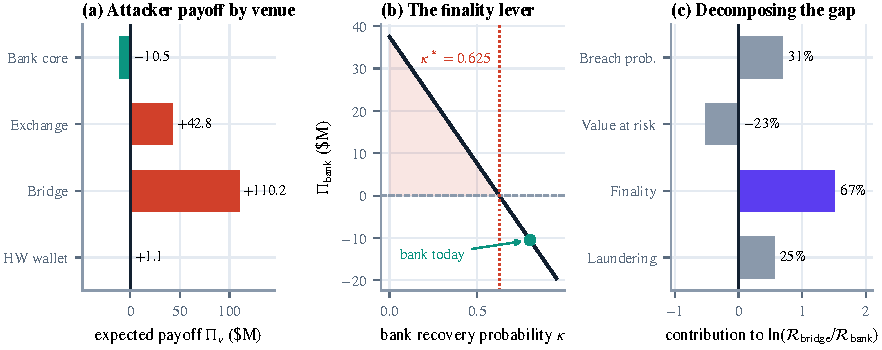
\includegraphics[width=\textwidth]{figures/fig2_attacker.pdf}
\caption{Attacker economics. (a) Risk-adjusted expected payoff $\Pi_v$ by venue, \cref{eq:payoff}. (b) The bank's payoff to an attacker as a function of its recovery probability $\kappa$; the bank is unattractive above the break-even value $\kappa^\ast$ of \cref{cor:breakeven}. (c) Exact decomposition of the log retained-value gap between bridge and bank, \cref{prop:decomp}; labels give each factor's share of the total.}
\label{fig:attacker}
\end{figure}

\subsection{Loss benchmarks and the compound-sum correction}\label{sec:benchmark}

In a 200{,}000-year run of the loss process, the mean annual loss is \ldaMean{} and the median \ldaMedian{}; the 95\%, 99\% and 99.9\% value-at-risk levels are \ldaVaRA{}, \ldaVaRB{} and \ldaVaRC{}, and the 99.9\% expected shortfall is \ldaESC{}, two and a half times the corresponding value-at-risk and close to the ratio $\alpha/(\alpha-1) \approx 2.67$ implied by a Pareto tail (\cref{fig:loss}). The truth used in the coverage study comes from a separate run of \TruthYears{} years: the 1-in-100-year annual loss is \truthC{}, the 1-in-1,000-year loss \truthK{}, and a year with losses of at least \$20 billion occurs on average once every \truthSys{} years, or with a probability of about half a percent per decade.

\Cref{app:shift} can be checked on the 200{,}000-year record. Above its 99.5th percentile (\fullU), the record contains \fullK{} exceedances, and the fitted shape is $\hat\xi = \fullXi$ (standard error \fullXiSE): with this much data, the estimate is precise but pulled below the planted \xiTrue{} by the log-normal body (\cref{rem:kink}). At $T = 100$ the incident-level return level \fullIncC{} misses the true annual level by \fullIncErrC\%; adding the mean annual loss of \fullShift{} gives \fullAggC, an error of \fullAggErrC\%. At $T=1{,}000$ the correction is only about 3\% of the level, and the remaining error (\fullIncErrK\% before, \fullAggErrK\% after) is governed by $\hat\xi$. This is the pattern \cref{eq:shift} predicts: the correction is first-order relevant at moderate return periods and second-order at long ones.

\begin{figure}[!tbp]
\centering
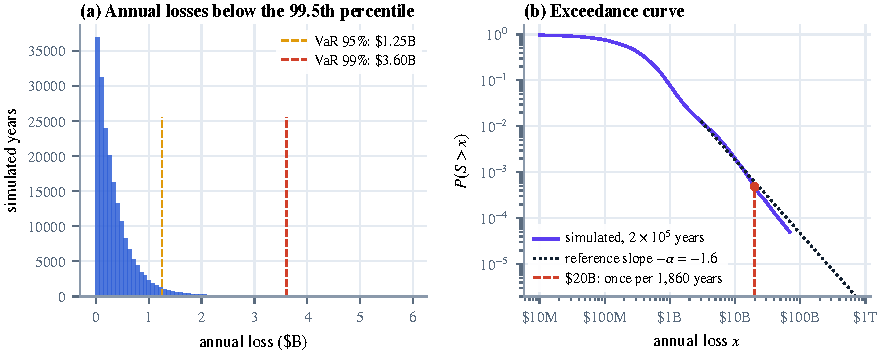
\includegraphics[width=\textwidth]{figures/fig3_loss.pdf}
\caption{The loss process. (a) Histogram of annual losses below the 99.5th percentile in a 200{,}000-year run, with value-at-risk levels. (b) Empirical exceedance curve on log--log axes; the dotted reference line has the planted slope $-\alpha$.}
\label{fig:loss}
\end{figure}

\subsection{What one record can and cannot reveal}\label{sec:single}

\Cref{fig:evt} shows inference from single records. Panels (a) and (b) use a 1,000-year record, more data than any real cyber-loss database. The mean-excess plot is close to linear, as a generalized Pareto tail requires, and the Hill estimate hovers near the planted $\alpha = 1.6$ over a range of moderate $k$. Yet the standard recipe of fitting at the 98th percentile places the threshold at \longU, just below the cascade trigger, and returns $\hat\xi = \longXi$ with a 95\% interval of $[\longXiLo, \longXiHi]$; the implied 1-in-1,000-year loss, \longPsi{}, is more than twice the truth. In the largest order statistics, where cascaded incidents dominate, the Hill estimate drifts towards one. A long record does not protect against a threshold placed on a kink.

Panel (c) uses a 100-year record with \shortK{} exceedances above \shortU{}, a typical draw with $\hat\xi = \shortXi$ close to the planted value. The point estimate of the 1-in-1,000-year loss is \shortPsi{} against a truth of \truthK{}. The three 95\% intervals are $[\shortDeltaLo, \shortDeltaHi]$ for the delta method, $[\shortBootLo, \shortBootHi]$ for the bootstrap and $[\shortProfileLo, \shortProfileHi]$ for the profile likelihood. All contain the truth here, but they disagree about where the uncertainty lies: the profile interval's lower limit is twice as high and its upper limit an order of magnitude higher. Panel (c) also exposes a pathology of the delta method. Its lower limit \emph{falls} as the return period grows beyond about a century, so that the lower confidence bound for the 1-in-10,000-year loss lies below the bound for the 1-in-100-year loss. This is the mechanical consequence of a log-symmetric band whose width grows faster than its centre. Profile limits are monotone in $T$, as they must be.

\begin{figure}[!tbp]
\centering
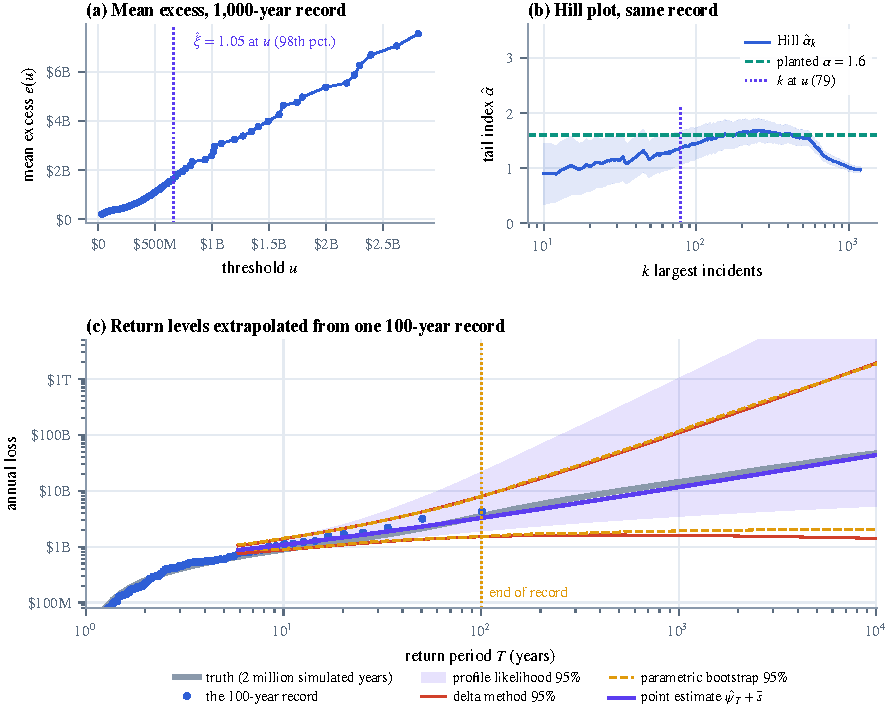
\includegraphics[width=\textwidth]{figures/fig4_evt.pdf}
\caption{Inference from single records. (a) Mean-excess plot of a 1,000-year record; the dotted line marks the 98th-percentile threshold. (b) Hill estimates $\hat\alpha_k$ with pointwise 95\% bands for the same record; the dashed line is the planted index. (c) Return levels from one 100-year record: the truth from \TruthYears{} simulated years, the record's own annual losses at their empirical return periods, the point estimate $\hat\psi_T + \bar s$, and 95\% intervals from the three methods.}
\label{fig:evt}
\end{figure}

\subsection{Coverage: how often is the truth inside?}\label{sec:coverage}

\Cref{tab:coverage} reports coverage for the 1-in-1,000-year loss, \cref{tab:misses} dissects the misses, and \cref{fig:coverage} shows all cells including $T=100$; \cref{tab:full} in the appendix gives every metric. Five findings stand out.

\emph{First, with records of realistic length the standard intervals fail.} In the full pipeline with 30-year records, the delta method covers the true 1-in-1,000-year loss \covBThirtyDeltaK\% of the time and the bootstrap \covBThirtyBootstrapK\%; with 100-year records these rise only to \covBHundredDeltaK\% and \covBHundredBootstrapK\%. The failure is not caused by misspecification: in Experiment A, where the model is exactly right, the delta method covers \covAThirtyDeltaK\% with 15 exceedances and \covAHundredDeltaK\% with 50. The parametric bootstrap, often recommended as a remedy, does no better: its coverage is within about two percentage points of the delta method's in every short-record cell.

\emph{Second, the failures are one-sided and dangerous.} Virtually every miss of the delta and bootstrap intervals lies wholly below the truth: \belowBThirtyDeltaK\% of delta intervals in the 30-year pipeline cell and \belowAThirtyDeltaK\% in the corresponding cell of Experiment A, with none lying above it (\cref{tab:misses}). These intervals do not merely understate uncertainty; they understate the loss.

\emph{Third, the cause is a downward-biased point estimate.} The median estimate of the 1-in-1,000-year loss is \medRatioBThirtyK{} times the truth with 30-year records in the pipeline and \medRatioAThirtyK{} times the truth in Experiment A, recovering to \medRatioAHundredK{} and \medRatioAThreeHundredK{} with 50 and 150 exceedances. The mechanism is the skewness of $\hat\xi$ in small samples from heavy tails: a short record rarely contains the extreme incidents that reveal how heavy the tail is, so $\hat\xi$ is below $\xi$ more often than not, and because $\psi_T$ increases steeply in $\xi$ when $\lambda_u T$ is large, $\operatorname{median}(\hat\psi_T)\approx\psi_T(\operatorname{median}\hat\xi) < \psi_T$. Any interval that is symmetric on the log scale around such an estimate inherits the bias.

\emph{Fourth, profile likelihood repairs most of the damage, and is better by a proper score.} Profile-likelihood intervals, which can be strongly right-skewed, cover \covBThirtyProfileK\% and \covBHundredProfileK\% in the 30- and 100-year pipeline cells and \covAThirtyProfileK\%, \covAHundredProfileK\% and \covAThreeHundredProfileK\% in Experiment A. Every short-record improvement over both alternatives is significant in a paired McNemar test ($p<0.001$). Coverage gains could in principle come from indiscriminately wide intervals, but the interval score rules this out: the profile likelihood roughly halves the mean score in the 30-year cells (\scoreBThirtyProfileK{} against \scoreBThirtyDeltaK{} for the delta method and \scoreBThirtyBootstrapK{} for the bootstrap in Experiment B) and has the lowest score in every cell of Experiment A. The price of honesty is width where data are thin: with 15 exceedances the median profile interval spans a factor of \ratioAThirtyProfileK{} from lower to upper limit, against \ratioAThirtyDeltaK{} for the delta method. With 150 exceedances the three methods converge (coverage \covAThreeHundredDeltaK\%, \covAThreeHundredBootstrapK\% and \covAThreeHundredProfileK\%; width ratios \ratioAThreeHundredDeltaK, \ratioAThreeHundredBootstrapK{} and \ratioAThreeHundredProfileK).

\emph{Fifth, no interval method fixes a biased threshold.} With 1,000-year records the threshold rule places $u$ near the cascade kink and the median estimate overshoots the truth by a factor of \medRatioBThousandK{}. The profile likelihood's misses then flip to the conservative side: only \belowBThousandProfileK\% of its intervals lie below the truth, and its coverage of \covBThousandProfileK\% is now significantly lower than that of the delta method (\covBThousandDeltaK\%), whose log-symmetric lower half happens to catch an overestimated level. The interval score agrees (\scoreBThousandProfileK{} against \scoreBThousandDeltaK{}). This cell is a reminder that interval calibration and threshold choice are separate problems: the first is solved by the profile likelihood, the second requires diagnostics and sensitivity analysis.

\begin{table}[!tbp]
\centering\small
\begin{threeparttable}
\caption{Coverage of nominal 95\% intervals for the 1-in-1,000-year loss}\label{tab:coverage}
\setlength{\tabcolsep}{5pt}
\begin{tabular}{@{}lrrrccc@{}}
\toprule
Experiment & $R$ (years) & $\bar k$ & Median $\hat\psi/\psi$ & Delta method & Bootstrap & Profile LR \\
\midrule
\tabinput{tables/tab_coverage_main.tex}
\bottomrule
\end{tabular}
\begin{tablenotes}\footnotesize
\item \emph{Notes:} Coverage in percent over \Reps{} independent records per row, with 95\% Wilson intervals in brackets. $\bar k$ is the mean number of exceedances; median $\hat\psi/\psi$ is the median ratio of the point estimate to the truth. Experiment A: exceedances exactly generalized Pareto with $\xi = \xiTrue$, truth \truthAK. Experiment B: full loss pipeline with thresholds at the 85th, 95th and 98th percentiles, truth \truthK.
\end{tablenotes}
\end{threeparttable}
\end{table}

\begin{table}[!tbp]
\centering\footnotesize
\begin{threeparttable}
\caption{Anatomy of the misses, 1-in-1,000-year loss}\label{tab:misses}
\setlength{\tabcolsep}{3.6pt}
\begin{tabular}{@{}lrrrrrrrrrrrr@{}}
\toprule
 & & \multicolumn{3}{c}{Below truth (\%)} & \multicolumn{3}{c}{Median upper/lower} & \multicolumn{3}{c}{Interval score} & \multicolumn{2}{c}{McNemar $p$} \\
\cmidrule(lr){3-5}\cmidrule(lr){6-8}\cmidrule(lr){9-11}\cmidrule(l){12-13}
Exp. & $R$ & Delta & Boot. & Profile & Delta & Boot. & Profile & Delta & Boot. & Profile & P vs D & P vs B \\
\midrule
\tabinput{tables/tab_misses.tex}
\bottomrule
\end{tabular}
\begin{tablenotes}\footnotesize
\item \emph{Notes:} ``Below truth'' is the share of intervals lying wholly below the true loss. The interval score is \cref{eq:score} on the $\log_{10}$ scale with $\alpha = 0.05$ (lower is better). McNemar $p$ is the exact two-sided $p$-value for the paired difference in coverage between the profile likelihood (P) and the delta method (D) or the bootstrap (B).
\end{tablenotes}
\end{threeparttable}
\end{table}

\begin{figure}[!tbp]
\centering
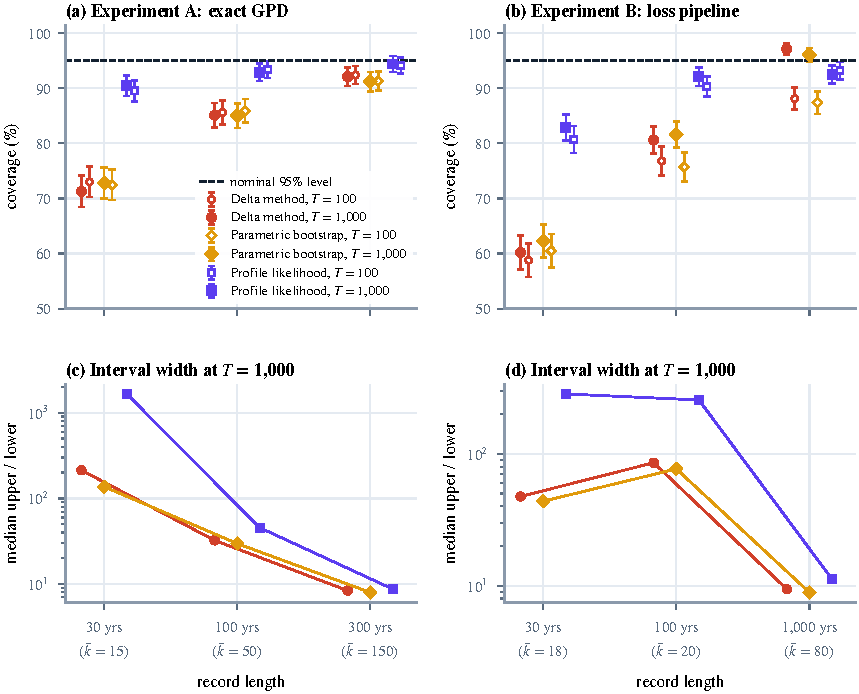
\includegraphics[width=\textwidth]{figures/fig5_coverage.pdf}
\caption{Coverage study. (a, b) Coverage of nominal 95\% intervals with 95\% Monte Carlo error bars, for $T = 1{,}000$ (filled) and $T = 100$ (open); the dashed line marks the nominal level. (c, d) Median ratio of upper to lower limit at $T = 1{,}000$ on a log scale. Experiment A fits a correctly specified tail above a known threshold; Experiment B runs the full pipeline on records from the loss process.}
\label{fig:coverage}
\end{figure}

\subsection{Contagion: a phase transition, and importance without size}\label{sec:res-contagion}

The exposure matrix of the network has $\rho(\Omega W) = \rhoOne$, so by \cref{prop:debtrank} shocks stop dying out once interbank exposure exceeds $\ell^\ast = \critExp$ times equity. \Cref{fig:contagion}a shows the transition. Below $\ell^\ast$ the contagion multiplier grows smoothly as the system approaches criticality; at $\ell^\ast$ it jumps by an order of magnitude and then saturates as every reachable bank defaults. At $\ell = 0.5$ a cyber event that wipes out 20\% of the largest bank's equity causes direct losses of \scBigDirect{} and total losses of \scBigTotal{} ($\Mult = \scBigMult$) without any default (\cref{tab:scenarios}). The same exposure scale makes a shared-vendor event benign: eight banks lose \scVendLowDirect{} directly and the system \scVendLowTotal{} in total. At $\ell = 1.2$, the vendor event destroys \scVendHighTotal, \scVendHighShare\% of system equity, and \scVendHighDef{} of the \nBanks{} banks default. The danger of concentration in third-party technology is not visible in calm, subcritical conditions; it materializes abruptly once leverage crosses a threshold.

\enlargethispage{\baselineskip}% final layout: lets the Discussion heading start on this page
Systemic importance, measured by the multiplier when a bank alone is hit, does not follow size (\cref{fig:contagion}b and \cref{tab:ranking}). The most systemic bank, \topOneName{} ($\Mult = \topOneMult$), is the smallest of the five core banks, and the second, \topTwoName{} ($\Mult = \topTwoMult$), is a periphery bank ranked \pOneSizeRank{}nd of \nBanks{} by assets that outranks \pOneBeatsCore{} core banks \pOneRatioLo{} to \pOneRatioHi{} times its size. The distinction between amplification and absolute impact matters here: a hit on the largest bank still produces the largest total loss (\scBigTotal{} against \cOneTotal{} for \topOneName{} and \pOneTotal{} for \topTwoName{}), but per dollar of direct damage, interconnection rather than size determines how far losses travel. Supervisory metrics that rank institutions by size alone will miss banks whose creditors are themselves thinly capitalized and densely connected.

\begin{table}[!tbp]
\centering\small
\begin{threeparttable}
\caption{Contagion scenarios (shock: 20\% of the equity of each bank hit)}\label{tab:scenarios}
\begin{tabular}{@{}lrrrrr@{}}
\toprule
Scenario & Direct loss & Total loss & $\Mult$ & Defaults & Rounds \\
\midrule
\tabinput{tables/tab_scenarios.tex}
\bottomrule
\end{tabular}
\begin{tablenotes}\footnotesize
\item \emph{Notes:} $\ell$ is the exposure scale; the critical value is $\ell^\ast = \critExp$. Total system equity is \sysEquity. Rounds count propagation steps until the relative change falls below $2\times10^{-4}$.
\end{tablenotes}
\end{threeparttable}
\end{table}

\begin{table}[!tbp]
\centering\small
\begin{threeparttable}
\caption{Most systemic banks by contagion multiplier ($\ell = 0.5$, 20\% equity shock)}\label{tab:ranking}
\begin{tabular}{@{}rllrrr@{}}
\toprule
Rank & Bank & Tier & Assets (\$B) & Size rank & $\Mult$ \\
\midrule
\tabinput{tables/tab_ranking.tex}
\bottomrule
\end{tabular}
\end{threeparttable}
\end{table}

\begin{figure}[!tbp]
\centering
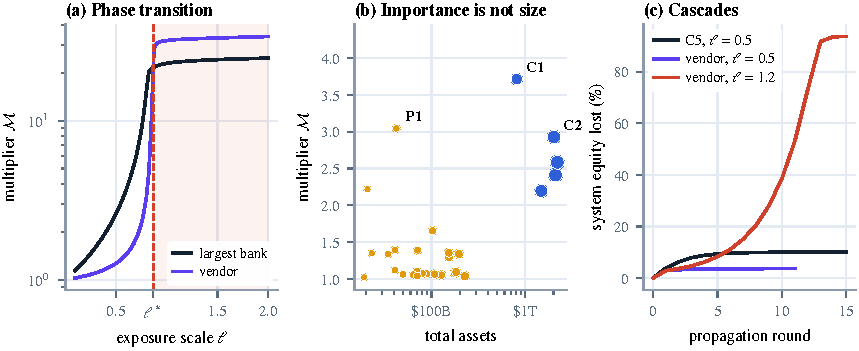
\includegraphics[width=\textwidth]{figures/fig6_contagion.pdf}
\caption{Interbank contagion. (a) Contagion multiplier $\Mult$ against the exposure scale $\ell$ for a hit on the largest bank and on a shared vendor serving eight banks; the dashed line marks $\ell^\ast = 1/\rho(\Omega W)$ and the shaded region the supercritical regime. (b) Multiplier when each bank alone is hit, against total assets; core banks in blue, periphery banks in amber. (c) Share of system equity lost by propagation round.}
\label{fig:contagion}
\end{figure}

\section{Discussion}\label{sec:discussion}

\paragraph{Reporting tail risk honestly.} The coverage study has a direct implication for how return periods of catastrophic cyber losses should be stated. With records of a few decades, the standard delta-method interval and its parametric-bootstrap substitute are not merely too narrow; they are centred on an estimate that is typically a fraction of the truth, and their misses all fall on the side that understates the loss. Statements of the form ``a loss of at least $x$ is expected once every $T$ years'' should therefore be accompanied by profile-likelihood intervals, and prudential uses should focus on the upper limit. Three further practices follow from our results. First, return levels should be reported across a range of thresholds, because, as \cref{sec:single,sec:coverage} show, threshold choice can bias estimates by a factor of two even with long records, and no interval method repairs that. Second, because the width of an honest interval shrinks rapidly with the number of exceedances (\cref{fig:coverage}c), pooling incident data across institutions and jurisdictions in supervisory or consortium databases has a high statistical return. Third, decision-makers should be told plainly what thin data imply: with 15 to 20 exceedances, an honest 95\% interval for the 1-in-1,000-year loss spans two to three orders of magnitude. A precise-looking estimate from such data should be read as a symptom of an overconfident method, not as information about the tail. Since capital and insurance premiums calibrated to a median-biased estimate will typically be too low, a supervisory margin over point estimates from short records is justified on statistical grounds alone.

\paragraph{Finality as a policy lever.} The attacker model suggests that the banking core is protected less by the difficulty of breaching it than by the reversibility of what an attacker can extract. Investments in payment recall, cross-institution freezing, anomaly-triggered settlement delays and international cooperation on tracing therefore carry a deterrence value beyond the losses they recover directly, because they remove the venue from the attacker's choice set (\cref{cor:breakeven}). Two corollaries deserve attention. First, the growth of instant, irrevocable payment systems raises finality inside the banking system itself. Our model predicts that, unless recovery mechanisms such as payee verification, reimbursement schemes or conditional delays restore the recovery probability, attacker effort will migrate towards these rails; this is a prediction of the model, not an empirical finding. Second, the asymmetry across venues is large. Because expected punishment and attack costs are small relative to retained value in crypto-asset venues, recovery alone deters attacks on the exchange only above a recovery probability of \breakEvenExchange{} (from \exchangeKappa{} in our calibration) and on the bridge only above \breakEvenBridge{} (from \bridgeKappa{}), against \breakEven{} for the bank. Issuer freeze functions, exchange cooperation and circuit breakers on bridges raise recovery, but at these levels attribution and sanction, the other terms of \cref{eq:payoff}, must do much of the work.

\paragraph{Interconnection and third-party concentration.} The contagion results imply that systemic cyber risk is strongly non-linear in interbank exposure. Below the critical exposure the system absorbs even large shocks with modest amplification; slightly above it, the same shock can destroy most of the system's equity. This argues for monitoring the spectral radius of the exposure matrix, or tractable proxies of it, as a macroprudential indicator, because the distance to criticality is more informative than the level of exposure itself. The ranking results argue for network-based measures of systemic importance alongside size-based ones, since a mid-sized periphery bank can transmit more loss per dollar of damage than most core banks. Finally, the shared-vendor scenario shows why third-party concentration deserves the supervisory attention it now receives \citep{dora2022}: in subcritical conditions a vendor compromise is benign, which is precisely why its danger is easy to underestimate, while near criticality it is the scenario that brings the system down. Stress tests that combine operational concentration with balance-sheet exposure, rather than treating them separately, capture this interaction.

\section{Limitations and extensions}\label{sec:limits}

\paragraph{Calibration.} Every parameter in this paper is illustrative. A calibrated version would estimate frequency and severity from operational-loss and incident databases, crypto-venue parameters from theft and recovery statistics such as those compiled by blockchain analytics firms, and the network from supervisory exposure data. The methodological conclusions depend on the tail index, the number of exceedances and the network spectrum rather than on dollar values, but their quantitative force in any application must be re-established with that application's data.

\paragraph{Stationarity and independence.} We treat years as independent and parameters as constant. Real cyber risk trends upward and clusters in campaigns that exploit common vulnerabilities. Both features would widen honest intervals further, so our coverage results are, if anything, optimistic. Self-exciting frequency models and time-varying severity are natural extensions.

\paragraph{Residual undercoverage.} With about 15 exceedances, profile-likelihood intervals still cover only about 90\%. A Bartlett correction of the likelihood-ratio statistic \citep{bartlett1937} or a bootstrap calibration of its distribution could close the gap; both are straightforward extensions of our code.

\paragraph{Threshold choice.} We fix thresholds by percentile rules, as practitioners often do. Automatic threshold selection, or models that span body and tail jointly, may reduce the bias documented in \cref{sec:single}.

\paragraph{Contagion mechanics.} Linear DebtRank passes equity losses through to claim values in full, which makes it an upper-bound stress test. Clearing models in the tradition of \citet{eisenberg2001} transmit losses only on default and imply much smaller amplification \citep{glasserman2015}; reality likely lies in between. We also omit liquidity and run channels, which \citet{duffie2019} and \citet{eisenbach2022} show can be first-order for cyber events that disrupt payments.

\paragraph{Attacker objectives.} The attacker model is static and risk-neutral, and it applies to financially motivated actors. State-sponsored attackers who seek disruption rather than profit are not deterred by finality, and they are arguably the more relevant threat for systemic events. The finality argument explains where profit-seeking attackers go; it does not imply that the banking core is safe from attackers with other objectives.

\paragraph{The compound-sum correction.} \Cref{app:shift} is derived heuristically and validated numerically; a proof under general regularity conditions, with a rate for the remainder, is left for future work.

\section{Conclusion}\label{sec:conclusion}

How bad, and how often? For the catastrophic cyber losses that worry supervisors, the honest answer from realistic data is a wide interval, and the intervals in common use are not honest. When a 1-in-1,000-year loss is estimated from 30 years of data, standard intervals miss the truth roughly 40\% of the time, always on the side that understates the loss, because the estimate they are centred on is typically a fraction of the true value. Profile-likelihood intervals restore most of the lost coverage and score better under a proper scoring rule, at the cost of upper limits that can be orders of magnitude above lower ones; that cost is the information content of the data, not a flaw of the method. Around this core result, we showed that the economics of attack are governed by finality, so that the banking core's main protection is the reversibility of what is stolen, and that losses which do land on banks propagate through interbank exposures with a sharp phase transition and with an importance ranking that size alone does not capture. All three findings point in the same direction: the quantities that matter most for systemic cyber risk are the ones a short record and a size-based view are least able to see.


\section*{Data and code availability}
All results are produced by an open Python package (\texttt{finality}) with a driver script that regenerates every table and figure from a single master seed (20261108). The package contains 19 unit tests, including a bit-exact cross-validation of the network generator against an interactive web implementation of the same models. The coverage study caches per-record intervals, so it can be resumed and audited record by record; on one CPU core the full study takes about five minutes. The scripts \texttt{paper/analysis.py} and \texttt{paper/make\_figures.py} produce all numbers quoted in the text, which enter the manuscript as generated macros rather than transcriptions; the figure script also runs an automated check that no text in any figure overlaps other text or plotted data.

\bibliographystyle{plainnat}
\bibliography{refs}

\appendix
\section{Derivation of the compound-sum correction}\label{app:derivation}

We give a heuristic derivation of \cref{app:shift}; a rigorous treatment of second-order asymptotics for random sums under general conditions is beyond our scope. Let $F$ have finite mean $\mu$, a regularly varying tail $\bar F(x) = x^{-\alpha}L(x)$ with $\alpha > 1$, and an eventually monotone density $f$, so that $f(x) \sim \alpha \bar F(x)/x$.

\paragraph{Fixed number of summands.} Let $S_n = X_1 + \dots + X_n$. For large $x$ the event $\{S_n > x\}$ is dominated by configurations in which exactly one summand is large \citep[Section~1.3]{embrechts1997}, so
\[
\Prob(S_n > x) \;=\; \sum_{i=1}^{n} \Prob\big(X_i + S_{n,-i} > x,\ S_{n,-i} \le x/2\big) + O\big(\bar F(x/2)^2\big),
\]
where $S_{n,-i}$ is the sum of the other $n-1$ summands and is independent of $X_i$. Conditioning on $S_{n,-i}$ and expanding $\bar F(x - s) = \bar F(x) + s f(x) + R(x,s)$ for $0 \le s \le x/2$,
\[
\begin{aligned}
\Prob\big(X_i + S_{n,-i} > x,\ S_{n,-i} \le x/2\big) ={}& \bar F(x)\,\Prob(S_{n,-i}\le x/2) + f(x)\,\E\big[S_{n,-i};\, S_{n,-i}\le x/2\big]\\
&+ \E\big[R(x,S_{n,-i});\, S_{n,-i}\le x/2\big].
\end{aligned}
\]
Because $\alpha>1$, the truncated mean converges to $(n-1)\mu$; the truncation error in the first term is $O(\bar F(x)^2)$; and the remainder is of order $\E[S_{n,-i}^2;\, S_{n,-i}\le x/2]\,|f'(x)| = O(x^{2-\alpha}\cdot x^{-\alpha-2}) = O(x^{-2\alpha})$, which is $o\{f(x)\} = o(x^{-\alpha-1})$ precisely when $\alpha > 1$. Hence
\[
\Prob(S_n > x) = n\bar F(x) + n(n-1)\,\mu f(x) + o\{f(x)\}.
\]

\paragraph{Poisson number of summands.} Mixing over $N \sim \mathrm{Poisson}(\lambda)$, and assuming the remainders are uniformly controlled, which the light tail of $N$ permits,
\[
\Prob(S > x) = \E[N]\,\bar F(x) + \E[N(N-1)]\,\mu f(x) + o\{f(x)\} = \lambda\bar F(x) + \lambda^2\mu f(x) + o\{f(x)\}.
\]
The identity $\E[N(N-1)] = \lambda\,\E[N]$ has a transparent meaning: given that a particular incident occurs, the remaining incidents of the year again form a Poisson process with intensity $\lambda$ (the Slivnyak--Mecke theorem), so the ``ordinary year'' that accompanies the big incident is an independent copy of $S$ with mean $\lambda\mu$. Reversing the first-order Taylor expansion,
\[
\lambda\bar F(x) + \lambda^2\mu f(x) = \lambda\big[\bar F(x) + (\lambda\mu) f(x)\big] = \lambda\,\bar F(x - \lambda\mu) + o\{f(x)\}.
\]
Setting $\Prob(S > \psi^S_T) = r_T$ and comparing with the incident-level definition $\lambda\bar F(\psi_T) = r_T$ gives $\psi^S_T = \psi_T + \lambda\mu$ up to terms of smaller order, that is, $\psi^S_T \approx \psi_T + \E[S]$. Because $\lambda\mu$ is fixed while $\psi_T$ grows like $T^{\xi}$, the relative size of the correction decays as $T^{-\xi}$, consistent with the numerical check in \cref{sec:benchmark}.

\section{Delta-method gradients}\label{app:gradients}

Write $m = \lambda_u/r_T$, so that $\psi_T = u + (\sigma/\xi)(m^{\xi}-1)$. For $\xi \neq 0$,
\[
\frac{\partial\psi_T}{\partial\lambda_u} = \frac{\sigma\, m^{\xi-1}}{r_T},\qquad
\frac{\partial\psi_T}{\partial\sigma} = \frac{m^{\xi}-1}{\xi},\qquad
\frac{\partial\psi_T}{\partial\xi} = -\frac{\sigma}{\xi^{2}}\big(m^{\xi}-1\big) + \frac{\sigma}{\xi}\, m^{\xi}\ln m ,
\]
and in the limit $\xi \to 0$, where $\psi_T = u + \sigma\ln m$, the gradient is $(\sigma/\lambda_u,\ \ln m,\ \tfrac12\sigma(\ln m)^2)$. The variance estimate is
\[
\widehat{\Var}(\hat\psi_T) = \Big(\frac{\partial\psi_T}{\partial\lambda_u}\Big)^{2}\frac{\hat\lambda_u}{R} + \bm{g}^{\top}\,\frac{1}{k}\begin{pmatrix} 2\hat\sigma^2(1+\hat\xi) & -\hat\sigma(1+\hat\xi)\\ -\hat\sigma(1+\hat\xi) & (1+\hat\xi)^2\end{pmatrix}\bm{g},\qquad \bm{g} = \Big(\frac{\partial\psi_T}{\partial\sigma},\frac{\partial\psi_T}{\partial\xi}\Big)^{\!\top},
\]
evaluated at the estimates, with the rate independent of the size parameters. The interval is formed on the log scale as described in \cref{sec:intervals}.

\section{Full coverage results}\label{app:full}

\begin{table}[!tbp]
\centering\footnotesize
\begin{threeparttable}
\caption{All coverage cells}\label{tab:full}
\setlength{\tabcolsep}{4pt}
\begin{tabular}{@{}lrrrlrcrrrrr@{}}
\toprule
Exp. & $R$ & $\bar k$ & $T$ & Method & Cov.\ (\%) & Wilson 95\% & Below (\%) & Above (\%) & Up/low & Score & $\hat\psi/\psi$ \\
\midrule
\tabinput{tables/tab_coverage_full.tex}
\bottomrule
\end{tabular}
\begin{tablenotes}\footnotesize
\item \emph{Notes:} \Reps{} records per cell, of which at least \minN{} yield an interval (records with fewer than eight exceedances are discarded). ``Below'' and ``Above'' are the shares of intervals lying wholly below or above the truth. ``Up/low'' is the median ratio of upper to lower limit; ``Score'' the mean $\log_{10}$ interval score of \cref{eq:score}; $\hat\psi/\psi$ the median ratio of point estimate to truth. No profile-likelihood interval was unbounded.
\end{tablenotes}
\end{threeparttable}
\end{table}

\section{Implementation and verification}\label{app:implementation}

\paragraph{Estimation.} The generalized Pareto maximum is located on a grid of 210 values of $\theta = \xi/\sigma$ spanning both branches, refined on an 81-point local grid with a parabolic polish, and compared with the exponential limit. The profile likelihood of the return level uses a $297 \times 9$ grid in $(\xi, \lambda_u)$ with separable parabolic refinement of the maximum; Brent's method locates each root of the likelihood-ratio equation to a tolerance of $10^{-4}$ in $\ln(\psi - u)$.

\paragraph{Unit tests.} Nineteen tests cover the package. They verify that the maximum-likelihood estimates recover known parameters and attain at least the log-likelihood of SciPy's optimizer for $\xi \in \{-0.2, 0.2, 0.625, 1.2\}$; that \cref{eq:rl} matches SciPy's generalized Pareto quantile function to a relative error of $10^{-12}$; that the EVT-implied return period inverts the return level; that all three intervals bracket the point estimate and that the profile interval is right-skewed for heavy tails; that delta and profile intervals agree within 5\% with 3{,}000 exceedances; that the Hill estimator recovers a planted Pareto index; that the threshold rule enforces the minimum number of exceedances; that the attacker decomposition is exact and the break-even recovery zeroes the payoff; that annual losses equal the sums of incident losses; and that DebtRank reproduces the closed form $(I-\Lambda)^{-1}h_0$ to $10^{-8}$ in the linear regime and produces defaults in the supercritical regime.

\paragraph{Cross-validation with the web instrument.} The network generator ports the companion web instrument's pseudo-random number generator bit for bit, with the same order of draws and the same stopping rule. A dedicated test pins the instrument's published numbers for seed 7: $\rho(\Omega W) = \rhoOne$; the three most systemic banks \topOneName{} ($\times\topOneMult$), \topTwoName{} ($\times\topTwoMult$) and \topThreeName{} ($\times\topThreeMult$); direct and total losses of \scBigDirect{} and \scBigTotal{} when the largest bank is hit; and a multiplier of \scVendHighMult{} with \scVendHighDef{} defaults for the shared-vendor scenario at $\ell = 1.2$. Two independent implementations, in JavaScript and Python, therefore agree on every contagion result reported here.

\paragraph{Reproduction.} Running \texttt{pytest} executes the tests in about one second, and \texttt{run\_study.py} reproduces every result from the master seed in about five minutes on one CPU core; its \texttt{budget} option splits the coverage study into resumable chunks whose per-record intervals are cached. The scripts \texttt{analysis.py} and \texttt{make\_figures.py} in the \texttt{paper} folder regenerate the tables, number macros and figures of this paper; the figure script replays the study's seeds, asserts that it reproduces the stored estimates exactly, and runs the automated overlap check on every figure.


\end{document}
